\documentclass[tikz,border=10pt]{standalone}
\begin{document}
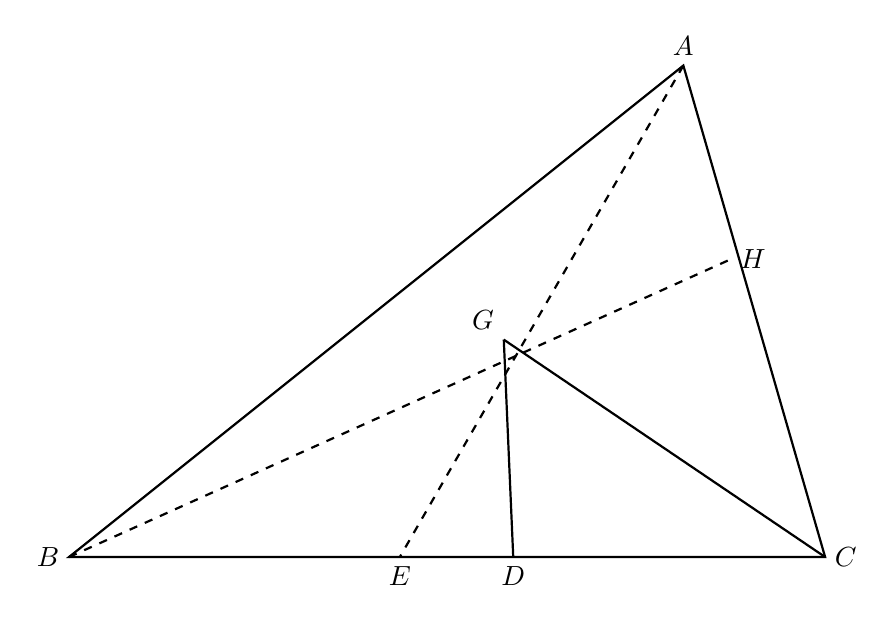
\begin{tikzpicture}[scale=1.2]
\coordinate (A) at (6.5,5.2);
\coordinate (B) at (0,0);
\coordinate (C) at (8,0);
\coordinate (E) at (3.5,0);
\coordinate (D) at (4.7,0);
\coordinate (G) at (4.6,2.3);
\coordinate (H) at (7.0,3.15);

\draw[thick] (A) -- (B) -- (C) -- cycle;
\draw[thick] (G) -- (D);
\draw[thick] (G) -- (C);
\draw[dashed,thick] (A) -- (E);
\draw[dashed,thick] (B) -- (H);

\node[above] at (A) {$A$};
\node[left] at (B) {$B$};
\node[right] at (C) {$C$};
\node[below] at (E) {$E$};
\node[below] at (D) {$D$};
\node[above left] at (G) {$G$};
\node[right] at (H) {$H$};
\end{tikzpicture}
\end{document}
